\documentclass[nofootinbib,UKenglish,nobalancelastpage,12pt]{article}
\usepackage[utf8]{inputenc}
\usepackage[T1]{fontenc}
\usepackage{babel, uiomasterfp}
%\usepackage{NotesTeX}
%\usepackage{layout}
\usepackage{subfigure}
\usepackage{tikz}
\usetikzlibrary{arrows}
\usepackage{multirow}
\usepackage{listings}
\usepackage{extarrows}
\usepackage{parskip}
\usepackage{eurosym}
\usepackage{float}
\usepackage{footmisc}
%\usepackage{kantlipsum}
\usepackage{algorithm}
\usepackage{algpseudocode}
\usepackage{hyperref}
% \usepackage{multicol}
\usepackage[a4paper,margin=1in,footskip=0.25in]{geometry}
%\usepackage[scaled=1.2]{mathptmx}
\DeclareSymbolFont{letters}{OML}{ztmcm}{m}{it}
\DeclareSymbolFontAlphabet{\mathnormal}{letters}
%\DeclareMathSizes{20}{20}{14}{10}
\newcommand{\vect}{\ensuremath{\mathbf}}
\hypersetup{
    colorlinks=true,
    linkcolor=blue,
    filecolor=magenta,      
    urlcolor=cyan,
    pdftitle={Overleaf Example},
    pdfpagemode=FullScreen,
    }

\bibliographystyle{plain}

\graphicspath{{figs/}}
%\newcommand{\includegraphicsmaybe}[2][]{\IfFileExists{../figs/#2}{\includegraphics[#1]{#2}}{\includegraphics[width=1\linewidth]{space_invaders.png}}}

%\renewcommand{\deg}{^{\circ}}
%\newcommand{\sn}{\sidenote}
%\newcommand\numberthis{\addtocounter{equation}{1}\tag{\theequation}}
%\newcommand{\hksqrt}[2][]{\ \mathpalette\DHLhksqrt{[#1]{#2\,}}}
%\def\DHLhksqrt#1#2{\setbox0=\hbox{$#1\sqrt#2$}\dimen0=\ht0
%    \advance\dimen0-0.3\ht0
%    \setbox2=\hbox{\vrule height\ht0 depth -\dimen0}
%    {\box0\lower0.65pt\box2}}
\usepackage{tikz}
\usepackage{listofitems} % for \readlist to create arrays
\tikzstyle{mynode}=[thick,draw=blue,fill=blue!20,circle,minimum size=22]
\begin{document}





\title{A big thanks to my supervisors Geir Storvik and Aliaksandr Hubin.}
\date{\today}
%\author{Leif-Martin Sæther Sunde}
\uiomasterfp[dept={Department of Mathematics},compact,date={\today},nosp, program={Stokastisk Modellering, Statistikk og Risikoanalyse},author=Leif-Martin Sæther Sunde,subtitle={Novel prior investigations},title = DAS MEISTERAUFGABE]




\maketitle

\tableofcontents
\clearpage
%\begin{abstract}
% Abstract

%\end{abstract}

% \begin{multicols}{2}
% \singlecolumn

% \section*{Abstract}\textit{
%     Everyone uses Gaussian priors in their BNNs. Maybe not the best idea. We tried something else, and our results have not necessarily developed to the hyperspherical priors advantage.}


%In not only modern machine learning, but all statistical prediction where datasets and computational recources are large, there seems to be a general case for the expansion of models fra beyond what was view as overfitting in the classical sense. (\textit{Belkin et al. 2019}\cite{Belkin_2019}) Where it seems like continually increasing the number of model parameters makes the test error "go beyond" overfitting, and slowly decreases even below the original classical best fit between underfitting and overfitting. However the regularization remains effective even as the number of parameters increase greatly.
\begin{center}
    

A quick note on terminology. In classical statistical learning the conventions for naming predictor and target variables varies. Predictor variables may be referred to by any of the following terms: "Covariate" (Continuous predictor varaibles) "Explanatory Variable" (Any predictor) "Confounding Variable" (Predictor variables that have dependency with other predictor varaibles).\cite{OBrien2020}\cite{Hastie2001}
\end{center}
\clearpage
\section{Background and Theory}
\subsection{Introduction}
We have a set of predictor variables in prediction modelling in general. As their names suggests, we hope are usable to predict another set of variables. Namely the target variables. In the classical statistical learning framework, we were historically working with datasets that by modern machine learning standards would be considered very small. This might be some of the reason for why the classical statistical learning framework developed as it did. Here it was assumed that usually the vast majority of the systematic relationship between predictor and target variables can be denoted with a model that has a limited amount of parameters, by modern standards. I.e. less than 50 for example.

Hence the systematic relationship is viewed as a largely tractable and human-interpretable relationship, the rest will in reality just be random noise. Therefore we wish to be careful with having a model with too many parameters and too high capacity. Since although this may lead us to achieve a lower error on our training data, It will yield us a higher error when we test our model on new data. Because the performance gain we saw on the training data was not caused by superior modelling of the true systematic relationship. Rather it was that our model was modelling the noise, or per haps even worse idiosyncratic noise, of our dataset. This effect is referred to as "overfitting". Hence the model should have a large enough number of parameters to adequately model the systematic relationship between predictor and target values, without having so many it captures the noise of our dataset.

%Often we don't know what parameters to include, so we will then include more parameters than we think is optimal and instead rather include a regularization term in the training of our model to induce sparsity. In general, we view the omission of parameters and addition of regularization as adding bias to our model, while adding more parameters as adding more variance to it. Therefore, finding the best compromise between the bias and variance has been called the bias variance tradeoff best-fit. 

Another way that is often used in practice to avoid having too high model variance, or overfitting, is regularization. Regularization is a part of a models architecture that aims to reduce variance, often by inclining the model to compress some of its parameters to, or close to, 0. Where 0 is a parameterstate such that the parameter does not influence the predictions of the model. 

In statistical learning it is common to employ more parameters than what is optimal on their own, and then add regularization. This is because this approach often results in lower test-error than the alternative. The view for why this is the case could be theorized as being because we don't exactly know what parameters, or kinds of relationships, there really are. Therefore we should let our model try a couple of them in order to adequately capture the systematic relationships. But then have the regularization there to avoid compounding several types of relationships into too complicated relationships, since we fear this will lead to overfitting. Therefore we allow to introduce this regularization bias, to have a greater reduction in variance of our model. Hence in the classical sense we wish to find the best tradeoff between bias and variance, by tuning the number of parameters and intensity of regularization. Therefore the best compromise between these two has classically been called the bias-variance tradeoff best-fit.

However, when computational recourses and datasets are large, there is evidence to suggest that the test error does not strictly follow this classical framework. We first observe the classical bias-variance-tradeoff curve, and then slowly as the number of parameters increase, the test error decreases. Even below the original bias-variance best-fit.\cite{Belkin_2019} Interestingly, this does not appear to mean going arbitrarily far in the variance direction in the classical sense either, since it is only the addition of parameters that lowers the test error. The regularization terms remain effective for arbitrarily large models. This is relevant for the work in this thesis, since, as our title "novel prior investigations", may suggest, one of our goals is to employ a more sophisticated form of regularization for these high-parameter models than what is usual for the field. The models most used in this new Machine Learning framework of \textit{More Compute} \cite{More_Compute} are based on the artificial neural network. \cite{LeCun1987}

As the reason for the drop of test error seems to be caused by the increase in parameters and complexity, and not the omission of regularization, it might be a good idea to try to bring the classical knowledge of statistical prediction into the modern machine learning world by looking at models that can be expanded to be arbitrarily complex, but with competent regularization. Setting the goal to  outperform the current combination of dropout layer by layer\cite{Srivastava2014} and $\mathcal{L}^2$  regularization pemalty parameter on the size of the whole parameter vector in the calculation of the loss. \cite{Wu2014} Since althogh $\mathcal{L}^2$ regularization has had good support in the classical learning litterature for a long time \cite{Marquardt_1975}, referred to there as "Ridge Regression", we aim to find room for improvement in both the dropout and $\mathcal{L}^2$ part simultaneously. 

However, these deep models have a tendency to on rare occasions fail spectacularly. Models that exert less of such behavior are in the litterature referred to as robust models. [Citation needed] These are of course in general desirable, with particular use in e.g. medical applications. In addition, the applications where robustness is especially desired, there is also often a desire for an unertainty estimate of the predictions the models make. This i a large part of the reason why classical statistical learning optimizing the bias-vairance tradeoff is still done regardless of its reduced performance when datasets and compute is readily avalible. Since although less performant overall in terms of test-error, these models are much more interpretable. Hence making an informed decision on how to treat their predictions and the uncertainty of those is much easier, in addition to their usual tendency to be more robust. 

An attempt to try to incorporate the best of both worlds, i.e. having the performance of high-parameter deep neural networks, with the uncertainty estimates and robustness of classical models is the Bayesian Neural Network. Bayesian Neural Networks have been shown to both match conventional neural networks, and outperform them in terms of robustness and uncertainty estimation, although at a greater cost of computation. \cite{current_BNN_infoandreviewGoan2020} Meaning they are usually only selected when datasets are small enough that computational recourses are sufficient regardless, or where uncertainty estimates are desired. Although the interpretability of classical models is still far out of reach for these models, the Bayesian Neural Network is aimed to compete with the conventional, or as we will adress them henceforth frequentist, neural networks. Which have the same problem of uninterpretablility. 

These usually employ a Isotropic Gaussian prior over their parameters. However, in this thesis we will attempt to find better priors that can hopefully replace the need for batch-normalization in an attempt to offset some of the increase in copmutational expense, and at the same-time hopefully be more computationally stable and informative.
\clearpage
\subsection{Frequentist Neural Networks}

The benchmark for the afforementioned high parameter models has for a while been the neural network. Although it has gone through many improvements over the years, and is more utilized as a module in modern larger architectures currently, is at its core the same as in '87. \cite{LeCun1987} However we will have to refer to these as frequentist neural networks (FNNs) for the remainder of this thesis, since we will explore novel solutions in the field of bayesian neural networks (BNNs).

We will begin by introducing a barebones FNN. It consists of alternating linear transformations and non-linear activation functions. The linear transformations are of the form $\textbf{x}^T\textbf{W}+\textbf{b}$ where x is the output from the previous activation function. The activation function is usually a ReLU function. Which applies to each of the elements $x_{i}$ in the output vector $\textbf{x}$ from the previous linear layer:

$$
g(x_{i}) = \max(0,x_{i}) =
\begin{cases}
0 & x_{i} < 0 \\
x_{i} & x_{i} \geq 0
\end{cases}
$$

The number of such layers are called the depth of the network. The outputdimension of each $\vect{W}$ (the $\vect{b}$'s are applied to the outputs so it's size always concides with the outputsize of $\vect{W}$) are referred to as the width of each layer $n$. Often this structure is visualized in a manner where the elements of the output from the activation layer are nodes and the linear transformation that follows as a set of connections between every previous node and every next node:

$$
[NN GRAPHIC]
$$

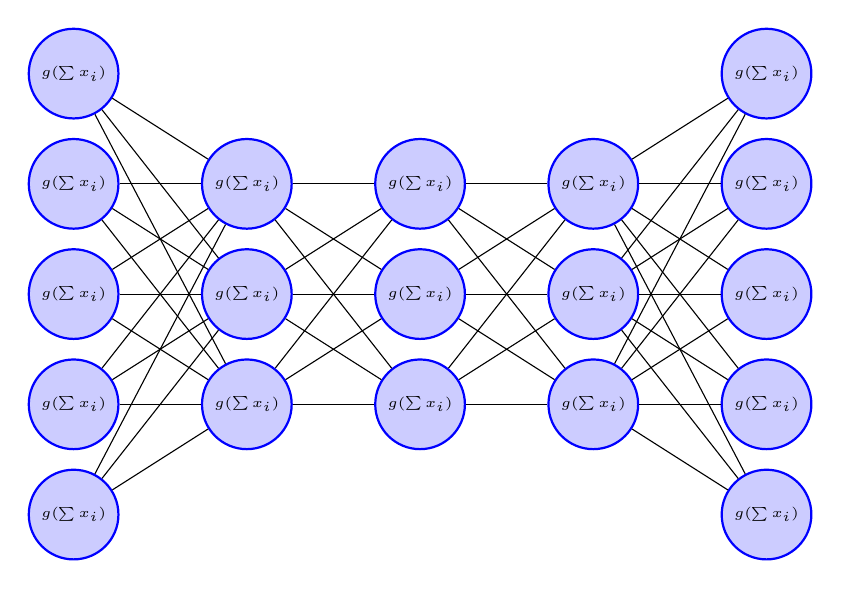
\begin{tikzpicture}[x=2.2cm,y=1.4cm]
  \readlist\Nnod{5,3,3,3,5} % number of nodes per layer
  % \Nnodlen = length of \Nnod (i.e. total number of layers)
  % \Nnod[1] = element (number of nodes) at index 1
  \foreachitem \N \in \Nnod{ % loop over layers
    % \N     = current element in this iteration (i.e. number of nodes for this layer)
    % \Ncnt  = index of current layer in this iteration
    \foreach \i [evaluate={\x=\Ncnt; \y=\N/2-\i+0.5; \prev=int(\Ncnt-1);}] in {1,...,\N}{ % loop over nodes
      \node[mynode, font=\tiny] (N\Ncnt-\i) at (\x,\y) {$g(\sum x_{i})$};
      \ifnum\Ncnt>1 % connect to previous layer
        \foreach \j in {1,...,\Nnod[\prev]}{ % loop over nodes in previous layer
          \draw[thin] (N\prev-\j) -- (N\Ncnt-\i); % connect arrows directly
        }
      \fi % else: nothing to connect first layer
    }
  }
\end{tikzpicture}
\clearpage
The trainable parameters here are the weights $\textbf{W}$ and biases $\textbf{b}$ of the linear part of each layer. The ReLU is not trained. By trainable we mean that these are the parameters updated when we fit our FNN to our training data. This procedure is done by first specifying a measure of how we wish to measure the "goodness of fit" of our model to the data, often RSS is chosen. This is then called the loss. Then a bootstrap sample of observations from our data set is sampled. Then the loss is calculated from this sample and the gradient of this loss with respect to the mentioned parameters is calculated. The gradient is calculated by invoking the chain-rule sequentially backwards through every layer. And then finally a small change in the parameters along the direction of the gradient is made. This process is referred to as stochastic gradient descent. \cite{Robbins1951} Exactly how large this change, usually called step, is is determined by the optimizing algorithm chosen. The optimizing algorithm usually tracks the direction of earlier gradients and makes larger steps if the gradients are calculated to roughly the same direction, and smaller steps if they are more different. The most common is called "Adam". \cite{Adam} These small steps are conducted several times, the exact number of times is usually referred to as epochs and is a tunable hyperparameter for the operator of the network.

\clearpage

\subsection{Bayesian Inference}
In the mathematics of Bayesian inference we assume there is a true model describing the entire systematic relationship between our target and predictor random variables. We also assume that this true model contains parameters, $\vect{\theta}$, but that these parameters are random variables, not real numbers. The random variable $\vect{\theta}$ has the distribution $p_{\vect{\theta}}(\vect{\theta})$. This distribution is called the prior. However, in the Bayesian framework, we also assume that the data $\mathcal{D}$ and parameters $\vect{\theta}$ are dependent random variables. Hence the distribution $p_{\vect{\theta}|\mathcal{D}}(\vect{\theta},\mathcal{D})$, which in Bayesian inference is called the posterior, is more informative than the prior on its own. Hence we invoke Bayes' Theorem to find it:

$$
%\mbox{\large
%$
p_{\vect{\theta}|\mathcal{D}}(\vect{\theta},\mathcal{D}) = 
\frac{ p_{\vect{\theta}}(\theta)p_{\mathcal{D}|\vect{\theta}}(\mathcal{D},\vect{\theta}) }{p_{\mathcal{D}(\mathcal{D})}}
%$}
$$

The term $p_{\mathcal{D}|\vect{\theta}}(\mathcal{D},\vect{\theta})$ is not neccessarily known, and classical statisticians often refer to the form of this distriution as "the model", however "likelihood" is also often used. This is the term we will utilize since it cannot be confused with the whole BNN/FNN itself. In practice the whole framework is probably at best an inaccurate simplification. And we do not know the prior either. However this prior should in theory represent the investigators prior beliefs about the parameter, hence the name. This prior belief is then updated by the observed data, $\mathcal{D}$, using Bayes' Theorem to find the posterior. 

Part of the case for conducting Bayesian inference over its frequentist counterpart, is firstly that if the parameters really are random variables, then of course the Bayesian Inference will be superior since in those cases the frequentist framework assuming the parameters are real numer will be wrong. However, even in the cases where the parameters might actually be real numbers, we can never know them exactly. Hence our uncertainty of them can be modeled by viewing this uncertainty as randomness, hence viewing the parameters themselves as random variables. Hence the Bayesian framework might better account for the uncertainty of parameters even if the parameters really are real numbers.
\clearpage
\subsection{Bayesian Neural Networks}

An already suggested way of bringing more competent regularization and better accounting for the stochasticity of the Networkparameters has been the introduction of Bayesian Neural Networks. These historically have employed a Isotropic Gaussian distribution over its parameters. Whether the biases are Gaussian aswell, or "frequentist" varies. In theory we want to update these distributions by calculating the gradient of the loss with respect to the parameters where the parameters are the weights and biases, and the theoretically ideal loss is the distance from the parameterposterior at that optimization step to the true parameterposterior given prior, model and data. We have from Bayes theorem that this is the true parameterposterior:

Let $p_{\vect{w}}$, $\vect{\theta}$, $D$ denote the prior on our weights (and possibly our biases aswell if these are also bayesian), the parameters of the distribution of the weights, and the data respectively. Let $\vect{w}$, , $p_{\vect{w}|D}$, $p_{D|\vect{w}}$ and $p_{D}$ denote the pdf's of the prior, posterior, likelihood and marginal of the data respectively. Note that in this framework, we are viewing our BNN as a perfect model of the relationship the entire systematic component between our predictor and target randomvariables, if it had the true posterior distribution over its weights and biases $\vect{w}$ when $\lim_{n \to \infty}$ (n is the number of observations, constituting $D$). We have from Bayes Theorem that:

%[OK hva foregår egentlig her? Hva menes med $p_{D|\vect{w}}$? Ser vi nå på datasettet vårt som jeg har beskrevet overnfor at den \textit{egentlige} modellen av dataen gitt prediktor variablene er faktisk BNN-et vårt. Ja det er akkuratt det, og fordelingen på den faktiske modellen av dataen er ikke bare beskrevet av BNN'et, men siden det også avhenger av den stokastiske variabelen W vill vi ha mer informasjon om hvor D trolig lander enn dersom vi ikke visste W. (Om vi ikke vet W kalles det marginalen.]

$$
p_{\vect{w}|\mathcal{D}}(\vect{w}, \mathcal{D}) = \frac{p_{\mathcal{D}|\vect{w}}( \mathcal{D},\vect{w})p_{\vect{w}}(\vect{w})}{p_{\mathcal{D}}(\mathcal{D})}
$$

Hence we do in fact have an expression in which we can in theory find the weights that maximize this expression, which would by definition be the maximum aposteriori solution. However, the term in the denominator requires us to solve an integral that is analytically intractable. Since we need to calculate this for every batch. Thus we would have to either use Markov-Chain Monte-Carlo (MCMC) to make an unrestricted estimate, or restrict the possible space of functions to approximate the true posterior pdf and assume this restriction sill contains a solution with satisfactory accuracy. A method that assumes such a restriction, greatly reducing computational cost and still having shown itself capable of modelling well is Variational Inference.

The prior, and usually the likelihood aswell, are almost always Gaussian just like the variational distributions of the parameters. (In fact, as they necessarily must be when the prior and likelihood are Gaussian.) A problem an acute reader who has never even heard of this architecture might already see is that how can you forward-pass and backward-pass through stochastic layers? The answer is that in each forward pass the BNN samples say 10 parametersamples from the distributions of each layer, and for each of those 10 samples it will insert the parametersample into the layers making and calculate a forward-pass as if it were an FNN with those parameters. After it has calculated those 10 different forward passes it usually calulates the average of them and delivers that final average as its prediction in the test case. The acute reader may then again consider that this must be substantially more comptationally expensive than the FNN and he/she would be right. The loss is not also directly and exactly calculated. Such a calculation would require an astronomically massive analytical solution for every gradient step. There are multpile ways of calculating such a loss. There are two ways of approximating this true posterior solution that are used in practice. One more precise and robust, and one more computationally affordable. Namely Markov-Chain Monte-Carlo (MCMC) and Variational Inference (VI) respectively.

So we want a type of regularization that is more competent on its own, but also in a manner that allows us to build our domain knowledge by specifying an appropriate prior on the parameter space. In addition the distributions on the parameters are also such that we think it better accounts for the uncertainty of the parameters in the classicly statistical sense. By this I mean that we view the whole network less as an actual AI and instead as is done in classical statistics, that it is simply a really complex model. In this view, lets assume that the true underlying model for the dependencies of our data is perfectly expressable with our model, then we it may be helpful to recognize the uncertainty in the estimates of our parameters, and hence our forward sampling and averaging will take better account for the uncertainty of the parameters and its mean-approximation could be suggested as to better have encapslated the uncertainty of our parameters than the standard dropout-stochasticgradientdescent-adam solution used more commonly. In addition Gaussian BNNs tend to not need dropout. There is empirical evidence suggesting this to be true \cite{Vincent_revisited}. 

It is hard to distill what of the reasons I have listed accounts for what increase in performance, but it seems that in general BNNs are more robust and outperform FNNs with the same number of nodes and depth. In addition to providing more accurate uncertainty estimates. However BNNs obviously also require more compute per depth than FNNs, so in the cases where we let the FNN have increased depth then if we have a large dataset then the BNN will tend to be somewhat less performant on average, but it retains an edge in robustness and uncertainty estimation. In cases where the dataset is small, the advantages magnify and the performance difference becomes smaller [citation of this.]

\subsection{Variational Inference}
If we do not have the computational recources for MCMC, we could try assuming a specific form of approximate posterior would work well. In variational inference we make this assumption, which allows us to greatly reduce the computational expense. We introduce the Variational distribution (abbrev.: VD, sometimes referred to as running posterior in the code.), which we specify the form of from the beginning. We then set the forward KL-divergence between our VD and the true posterior as the loss we wish to minimize.

The $\vect{\theta}$ in $q_{\vect{\theta}}$, is there to denote the parameters in our VD.

Let $q_{\vect{\theta}}$ denote the pdf of the VD. The parameters $\vect{\theta}$ in the VD are what is actually updated at each gradient step. If our assumption regarding the VD is in fact correct, then modern optimization regimes like f.ex. adam [adam citation] should leave us with a reasonably low loss after a while, which will neccessarily imply at the least low training error.

Minimizing the KL-distance between our VD and the true posterior is made much easier by rearranging some terms:

$$
\begin{aligned}
& K L(q_{\vect{\theta}}(\vect{w}) \, || \, p_{\vect{w}|\mathcal{D}}(\vect{w},\mathcal{D}))
& \stackrel{def}{=}\int q_{\vect{\theta}}(\vect{w}) \log (\frac{q_{\vect{\theta}}(\vect{w})}{p_{\mathcal{D}|\vect{w}}(\mathcal{D},\vect{w})}) \,d \vect{w}
\end{aligned}
$$

We then invoke Bayes Theorem on $p_{\vect{w}|\mathcal{D}}(\vect{w}, \mathcal{D})$:

$$
\begin{aligned}
& =\int q_{\vect{\theta}}(\vect{w}) \log (\frac{q_{\vect{\theta}}(\vect{w})}{\frac{p_{\mathcal{D}|\vect{w}}(\mathcal{D},\vect{w}) p_{\vect{w}}(\vect{w})}{p_{\mathcal{D}}(\mathcal{D})}}) \,d \vect{w} \\ 
& =\int q_{\vect{\theta}}(\vect{w})(\log (\frac{q_{\vect{\theta}}(\vect{w})}{p_{\vect{w}}(\vect{w})})-\log (p_{\vect{w}|\mathcal{D}}(\vect{w}, \mathcal{D}))+\log (p_{\mathcal{D}}(\mathcal{D})) \,d \vect{w}
\end{aligned}
$$



$$
=\int q_{\vect{\theta}}(\vect{w})(\log (\frac{q_{\vect{\theta}}(\vect{w})}{p_{\vect{w}}(\vect{w})})-\log (p_{\mathcal{D}|\vect{w}}(\vect{w}, \mathcal{D}))) \,d \vect{w} +\int q_{\vect{\theta}}(\vect{w}) \log (p_{\mathcal{D}}(\mathcal{D}))\,d\vect{w}
$$

$$
=\int q_{\vect{\theta}}(\vect{w})(\log (\frac{q_{\vect{\theta}}(\vect{w})}{p_{\vect{w}}(\vect{w})})-\log (p_{\mathcal{D}|\vect{w}}(\vect{w}, \mathcal{D}))) \,d \vect{w} + \log (p_{\mathcal{D}}(\mathcal{D})) \int q_{\vect{\theta}}(\vect{w}) \,d\vect{w}
$$

The last integral will sum to 1, since it integrates a pdf over its entire domain.

$$
=\int q_{\vect{\theta}}(\vect{w})(\log (\frac{q_{\vect{\theta}}(\vect{w})}{p_{\vect{w}}(\vect{w})})-\log (p_{\mathcal{D}|\vect{w}}(\vect{w}, \mathcal{D}))) \,d \vect{w} + \log (p_{\mathcal{D}}(\mathcal{D}))
$$

Note that the logmarginal density of D, $\log{p_{\mathcal{D}}(\mathcal{D})}$, will not change as we update $\vect{\theta}$. Hence minimizing this term above will be equivalent to minimizing the term below:

$$
=\int q_{\vect{\theta}}(\vect{w}) \log (\frac{q_{\dot{\theta}}(\vect{w})}{p_{\vect{w}}(\vect{w})}) \,d \vect{w}-\int q_{\vect{\theta}}(\vect{w}) \log (p_{\mathcal{D}|\vect{w}}(\mathcal{D},\vect{w})) \,d \vect{w}
$$

%[Add a final part where we convert to expectations?]

%[Remember that this framework you have written is not SGD, or even using batches of the data for training. You are using the entire dataset as your batch everytime.] But am I really though, I have just specified the form of the loss here..

Conventionally the minuend and subtrahend are called the KL-terms and Reconstructon terms respectively. This is because the the first term coincides exactly with the definition for the forward KL-loss between our prior and our VD, while the second term coincides exactly with the expectation of the liklelihood of our data. Hence a useful interpretation, more often used as the interpretive framework than the minimizing of distance between VD and true posterior, is to view the KL-term as the regularization term and the reconstruction loss as analogous to traditional RSS loss.

The KL-loss here can be viewed as a regularization parameter that replaces the $\mathcal{L}^2$ loss term in FNNs. We hope that this regularization will also be a more appropriate regularization than the $\mathcal{L}^2$, since we can make a more specific prior distribution that the parameters are regularized towards, rather than just inducing a bias to reduce parameter distance from 0. Our hope is that we can find a prior such that the parameter space is regularized towards something more helpful.

Luckily, both of theese terms can be easily approximated with reasonable accuarcy through Monte Carlo approximation. (The precision of which is denoted by enums in the code.) This Monte Carlo approximation is done by making a sample from $\vect{\theta}$, which we have approximated the pdf of $q_{\vect{\theta}}$, and then conducting a forward pass with those realized weights $\vect{w}$ and calculate the loss in our earlier expression for each of theese iterations. This process is repeated enums times before we average the losses we computed as our final loss we wish to minimize.


Variational inference is a technique for approximating the posterior, which is less precise than MCMC, but saves a lot of computation. Mathematically we are minimizing the KL divergence, a statistical distance for probability distributions, between our posterior and the true posterior. Minimizing this distance can be shown to be equivalent to minimizing the KL divergence between our approximated posterior and the prior and maximizing the likelihood \cite{VI_paper}. 

\section{Novel Priors and Variational Distributions}

A problem for deep neural networks in general, is that of exploding and vanishing signal, both in the forward pass and in the gradient backward pass. The conventional way of addressing this, when the nets are deep enough for this to be an issue, is to employ batch-normalization. Batch normalization\cite{Batch_Norm_original} is a technique where in between every, or every-so-often, layer we normalize the norm of the forward passing vector to be one. This is also done for the conventional Gaussian prior and VD BNNs. However, something new to consider is what if the distributions of our VD and prior are constructed in such a manner that the norm of every forward pass is 1? In theory this could save computation if those distributions are not too much more expensive computationally than the Gaussian. However, we wish to also retain as much as possible of the properties in the Gaussian distribution, since it has as mentioned earlier reasonably good performance and seems already to replace the need for dropout. 

Hence we introduce the combination of a von Mieses-Fisher (vMF) VD and HypersphericalUniform (HU) prior. Theese distributions do have the property of having norm one, while also being closely related to the Gaussian distribution.

\subsection{Hyperspherical Uniform Prior}
A class of priors and VD's suggested recently is the radial directional distribution. \cite{Vincent_review}
\begin{equation}
    \vect{w} = w_r\vect{w}_d, \hspace{4mm} w_r \sim p_{\text{rad}}\left(w_r\right) \hspace{4mm} \vect{w}_d \sim p_{\text{dir}}\left(\vect{w}_d \right).
\end{equation}
This distribution separates the direction from the magnitude, hence making them separately trainable. However, since we would like to replace the need for batch-normalization we set the radial component $\theta_r = 1$, we place our prior and VD on the norm 1 hypersphere. Meaning all our weights in every forward pass will have norm one.

Since I don't see any good reason to introduce a bias in any direction on the hypersphere, we use an uninformative prior for the directional component, i.e. the uniform, yielding the Hyperspherical Uniform prior. This should make each forward pass pass its vector on, with the norm of the vector remaining the same and in theory, remove the need for batch-normalization. The posterior distribution that follows from this is the Von Mieses-Fisher distribution, which can be seen as the hyperspherical extension of the normal distribution. Hence we hope that our prior will inherit the benefits of the Gaussian prior, while adding the benefit of replacing batch normalization.

% In addition to replacing batch normalization the posterior, Von Mieses-Fisher, which is a generalization of the Gaussian distribution inherits its useful properties. Namely a regularization that has shown itself useful before in Gaussian BNNs, replacing the need for $\mathcal{L}^2$ regularization with a perhaps even more helpful one. 
In addition to this, the stochastic nature of the net is obviously preserved. In each forward pass the size of each weight varies, meaning some of the connections become very unimportant, similarly to dropout. This means that the effect of forcing learning across several of the connections is preserved, thus also replacing dropout just like conventional Gaussian BNNs do.

Lastly, recent results indicate that a Variational Autoencoder with a Hyperspherical Uniform prior for density estimation over a dataspace with latent hyperspherical structure can perform better than its Gaussian counterpart \cite{VAE_vmf_paper}. We have not investigated the effect of this possible advantage in our datasets.

\subsection{The Von Mises-Fisher Variational Distribution}
The probability density function of the von Mises Fisher distribution for the random p-dimensional unit vector ${\displaystyle \mathbf {x} }$  is given by:
$f_{p}(\mathbf{x}; \boldsymbol{\mu}, \kappa) = C_{p}(\kappa) \exp \left( {\kappa \boldsymbol{\mu}^\mathsf{T} \mathbf{x} } \right)$ where $C_p(\kappa)$ is defined by

$$
C_{p}(\kappa )={\frac {\kappa ^{p/2-1}}{(2\pi )^{p/2}I_{p/2-1}(\kappa )}}
$$
where ${I_{\nu}}$ denotes the modified Bessel function of the first kind at order ${\nu}$.

the normalization constant reduces to
$$
{\displaystyle C_{3}(\kappa )={\frac {\kappa }{4\pi \sinh \kappa }}={\frac {\kappa }{2\pi (e^{\kappa }-e^{-\kappa })}}.}
$$

with parameters $\boldsymbol{\mu}$ and $\kappa$ as the mean direction and concentration parameter. The greater the value of $\kappa$, the higher the concentration of the distribution around the mean direction $\boldsymbol{\mu}$. We can therefore view this parameter as a type of variance, although this is strictly speaking only a parameter of variance in the directionalcomponent, not the radial. As the norm will always be 1.

Since we would like to keep computational cost as low as possible, avoiding both batchnormalization and dropout is helpful. Although it must be said that neither of them are too intensive, especially dropout, so even with this novel VD-prior combination we will still have an architecture significantly more expensive per depth than its frequentist counterpart.

\subsection{The two von Mieses-Fishers}

One way of implementing our VD and prior is to make all the weights in each layer be drawn from a single von Mieses-Fisher random variable. This results in performance 20 percent worse than the Gaussian, which I believe is due to the excessively strong regularization that this imposes on each entire layer. Analogously to what happens in ridge regression when the regularization parameter there is so strong that only the mean, $B_{0}$ is found and all other covariates regress to 0. 

However, a second way to implement it is to have each recieving node in the network have weights drawn from a vMF. This results in much better performance, since the regularization is weaker. However the gradient is still kept within bounds, better than its Gaussian counterpart.

\section{Results}

The HU-vMF combo seems susceptile to regress to only predicting the mean of its target value, this is known as a pathological posterior collapse. However measures can prevent this.

\section{Reproducibility}

I will open this section with a bold statement. "Nonreproducible science" is an oxymoron. 

\subsection{Terminology}

Confounding use of terminology is a problem in scientific publications across disciplines in general, and is of particular concern here.
A first group use replicable to denote  “same data+same methods=same results,” and reproducible to denote “new data and/or new methods in an independent study=same findings”. While a second group swap the two terms. And of course, there is a third group that makes no distinction between the two terms at all. This problem is well adressed by \cite{Barba_2018}. I will use what is  called the Claerbout-Donoho-Peng convention there. Where the terms follow the definitions from the first group

\subsection{The Philisophical Foundation of Science}

A definition of science from [Oxford Languages] reads as follows:

the intellectual and practical activity encompassing the systematic study of the structure and behaviour of the physical and natural world through observation and experiment. 

This definition could have been better in my opinion, since it does not specify what it means by "systematic". If we would look at potatoes while thinking about them. Occasionally pick them up, and then drop them again. And then concluding the moon indeed is flat. Repeating this procedure several times in a row would satisfy \textit{a} systematic study of the structure and behaviour of the physical and natural world through observation and experiment. However, we could all agree that would not really be science. Or at the very least, not optimal science.

Fully fleshed out, the systematic part of the definition refers to the fact that we observe the world with a hypothesis that is well formulated in our currently proven or assumed body of scientific truths. We then observe nature either as is, or in an experiment we fashion. Then, again using the framework of previous science to interpret theese results, we evaluate whether or not we think the observations support or contradict our hypothesis. In 1600 we would now be done, and certain parts of the scientific community could through scientific observation seem to think the same, however, we aren't. In order to decide whether or not this hypothesis or its rejection should be incorporated into our body of scientific knowledge, there must be a converging body of evidence from several indepentent studies. If this happens, then we are actually done and the knowledge is admitted.

\subsection{Importance of Reproducibility for Modern Science}

If I were to observe my hand closing at the same time as the rain stops, everyone would agree that that is insufficient evidence for concluding my hand closing has correspondence with cessation of rain. Therefore the scientific community should drop what they are doing and investigate my hand instead, right? No. I should instead myself several times in different setting and aggregate my observations to a dataset and statistically evaluate my findings. Now, if I report a that the correspondence is genuine and with a summary of my investigation of the data and the methods used in my code. This time the scientific community should drop what they are doing and investigate, right? No! The \textit{least} I could do to limit how much I am asking for the scientific community to trust me, aswell as help them evaluate the validity of my investigations without too much effort from their part. This is where reproducibility comes in. If I make all my code and data open and avalible (how to best solve the code part in practice is discussed later) in order to let them check one of the parts of the scientific process that is \textit{the most prone to error} [MOST PRONE TO ERROR PAPER] for themselves quickly. Where they can see after two seconds that I had mistaken my index-column for my "number of occurences of rain-cessations"-column, and that my data actually indicated no correspondence. This is of course a construced example, however there are real examples of very close to this last mentioned error [THE INSANE MEDICAL EXCEL FILE GUY], only in reality it was even worse since the publications were in fact peer-reviewed before publication and it still slipped through.

Therefore it comes to us, the scientists, to the best of our ability, be humble and industrious enough to allow such errors to be detected early on and improve the scientific quality of our knowledge. However that is not all, in addition to that other scientists may make findings in the investigations of our data that we missed! Knowledge they extract for us original publishers, that would have remained hiden for humanity for ever otherwise. Or that they may use parts, or all of, our code in useful computational tools for science, education or industry later on. How to do this in practice is elaborated on in the next subsection, where "computational reproducibility" is a shorthand referring to reproducibility of both code and data.

\subsection{Computational Reproducibility in Practice}

Reproducibility is a term that is not relevant for all the stages of the scientific process. However, in most modern science, there will be data and code involved. From that point onwards, reproducibility is an effort that provides far more reward than it requires investment. 

Since github tracks all changes when used correctly, it is possible to see for other scientists whether you made some erroneous formatting choices or changes to your data. 

Conda environments, also when used correctly, allows other scientist to make their computer work in the same way as the computer of the original publisher, which is essential for making it easy for them to rerun and edit your code.

Jupyter notebooks, optimizes this even further. If we also use Bindr, then we can also facilitate inclusion of all the talent from the less eonomically fortunate scientists. By greatly reducing the need for computational recoures required to rerun and edit the code and/or data. AI tasks are of course much more difficult, although letting everyone retrain the model in any reasonable timeframe is too ambitious for bindr, we could still instead load a pretrained model into the notebook, which could allow others to add transformations or test-case hypermarameter modifications to the AI.

Not only that, but this coputational framewrok has the added benefit of not only greatly accomodating scientific collaboration after publication, but also during the scientific work leading up to the publication itself. It in fact accomodates collaboration between a lot of scientists. This is, in my view, the future. A group with great, smooth collaboration will always outperform any individual.

\section{Experiments}

For the experimental design to test the efficacy of our vMF BNN vs the conventional Gaussian BNN, we are designing experiments with 4 datasets. In three of them we will test classification performance, where one of them will also support evaluation of uncertainty estimation performance, and one regression dataset. 


\subsection{Phoneme data}
The first classification experiment is with the phoneme dataset \cite{phoneme_MAYBEWRONGLOOKINTOIT} [THIS CITATION COULD BE INCORRECT]. Here we train ten Gaussian and ten vMF BNN's. They get to train on a random sample of about three quartes of the data, and then we find the average accuracy of the 10 Gaussian and 10 vMF nets on the remainign unseen quarter of the data.

\subsection{Simulated Data}

Here we generate samples from 5 bivariate Gaussian distributions. These are consciously made in a way that the classes overlap with each other in some areas, while in other areas it should be pretty clear where a sample was drawn from. 

We conduct the same train and test and 10 network training regimen as in the phoneme data. However here we also evaluate the efficacy of the uncertainty estimation of the Gaussian BNN vs the vMF BNN. This is conducted by calculating the cross-entropy [MATHEMATICAL FORMULA] of each model along the entire 2D domain of the bivariate Gaussian distributions. We hope to see the nets be confident around the edges of the plot, but to have a "diamond" of uncertianty around the middle Gaussian distribution, aswell as four lines of uncertainty dividing the other 4 distributions, these lines should extend indefinitely long.

\subsection{Regression with Carbon Nanotubes Data}

We used the carbon nanotubes data here from the UCI library, as we used in the project published at berkeley.\cite{CarbonNanotubes} This dataset is has the desirable qualities of having not too many covariates, while also having more than ten thousand observations. In addition to being not too easy to predict. 

We follow a similar regimen to our classificaion tasks, although now we measure the each of the ten-net ensembles in mean suqared error instead of measuring in average number of correct classes predicted.
\clearpage
\section{Discussion}

\subsection{Implementation Issue}
A problem with my implementation of the HU-vMF combo, is that in my implementation I have not succeeded in calculating a gradient in the actual domain of our vMF, e.g. on the norm 1 hypersphere. Instead pytorch thinks that the mu's of the vMF need not be normalized, and then it takes a gradient step along its registered mu in the direction it thinks reduces the loss, disregarding the norm 1 constraint. Then for actually calculating the loss and making the samples for the forward passes, we then after-the-fact normalize our mu to be on the domain of our vMF. This is not a good solution, and is in my view the main current weakness of my implementation. I am convinced is significantly hurting performance, especially when the number of observations and epochs gets large. I belielve this might even be causing so much harm, that had it been resolved the vMF might consistently outperform its Gaussian counterpart in every task.

In addition there is also a mathematical issue with the von Mieses-Fisher distribution itself, namely that it has one variance for all its components. Per haps this is the only way to tractably achieve norm 1 weight and bias samples, as I can imagine a pdf that has this property \textit{and} individual variance along each component to be even more complicated than the von Mieses-Fisher is, however I suspect this is a substantial weakness. One could argue that this could help reduce overfitting, as one could view it as a form of competent regularization, but even thogh I have reason to argue positively for my own project I must confess I view it as much more of a weakness than a strength. Furthermore I also believe this is part of the reason why the nodewise von Mieses-Fisher architecture is superior to the layerwise von Mieses-Fisher. 
\clearpage

\bibliography{refs}

\end{document}
